\section{Introduction}
This document describes the System, Integration, and Unit Test Plan (SIUTP) for
\progname{}. Its purpose is to describe the testing efforts to verify the
ability of \progname{}'s implementation to meet its functional and
nonfunctional requirements as described in its Software Requirements
Specification (SRS, Version~\srsVersion) and additional data types and models
as described in its Module Guide (MG, Version~\mgversion) and Module Interface
Specification (MIS, Version~\misversion). This also acts as a basis for
regression testing as \progname{} is developed further. It describes tests for
each requirement and module, traceability between tests and \progname{}'s
requirements, and testing and verification tools.

This test plan does \textit{not} include validation efforts to evaluate
\progname{}'s acceptability for its end-users and stakeholders. That
information is in its Acceptance Test Plan (ATP).

The document's content and organization is loosely based on IEEE Std 829-2008
Clause 9: Level Test Plan (LTP)~\citep{vvDocIEEE}.

\subsection{Summary of \progname{}'s Purpose and Design Goals}
\progname{} is a Computational Model of Emotion (CME) for Non-Player Characters
(NPCs) to enhance their believability, with the goal of improving long-term
player engagement. \progname{} is for \textit{emotion generation}, accepting
user-defined information from a game environment to determines what emotion and
intensity a NPC is ``experiencing''. How the emotion is expressed and what
other effects it could have on game entities is left for game
designers/developers to decide.

\progname{} aims to provide a feasible and easy-to-use method for game
designers/developers to include emotion in their NPCs, they perceive to be
challenging with the current tools and
restrictions~\citep{broekens2016emotional}. \progname{} should be modular and
portable such that game designers/developers can use it in their regular
development environment, and should not require knowledge of affective science,
psychology, and/or emotion theories. Therefore, it is a library of components
to maximize a game designer/developer's control over how and when \progname{}
functions.

\subsection{Scope of Testing Efforts}
The overall goals of \progname{}'s system, integration, and unit testing effort
are:
\begin{enumerate}

    \item Ensure traceability between \progname{}'s verification efforts and
    its SRS, MG, and MIS

    \item Build confidence in the correctness and accuracy of \progname{}'s
    source code

    \item Build confidence in \progname{}'s overall verification efforts

\end{enumerate}

This test plan must be \textit{reviewed} for each new major version of
\progname{}'s SRS, MG, and/or MIS and revised accordingly. This ensures that
these testing efforts remain relevant throughout \progname{}'s development. For
new minor versions of \progname{}'s SRS, MG, and/or MIS, the review can be
limited to only those sections related to SRS, MG, and/or MIS modifications to
help reduce the effort required when testing the next major version.

This test plan must be \textit{executed} in full for each new major version of
\progname{}'s source code. Previous versions do not need to be retested. The
SIUTP can be partially executed for new minor versions of the source code to
help reduce the effort required when testing the next major version.

The SIUTP describes the ``Dynamic Testing Method'' for Implementation
Verification referenced in \progname{}'s Master Test Plan (MTP)
Section~\ref{plan:implementation}.

\subsection{Project Organization}
\progname{}'s development uses the general software development life cycle
processes of requirements analysis, architecture and design definition,
implementation, verification, and validation. Each of these processes outputs at
least one Software Development Artifact (SDA) which serves as a description of
the process's results and becomes an input to subsequent processes
(Figure~\ref{fig:dependencies}). Each SDA has an associated verification and/or
validation plan (Table~\ref{tab:verificationPlanLocation}) to ensure that it
adheres to the \progname{}'s concept.

\vspace*{\fill}
\begin{figure}[!h]
    \centering
    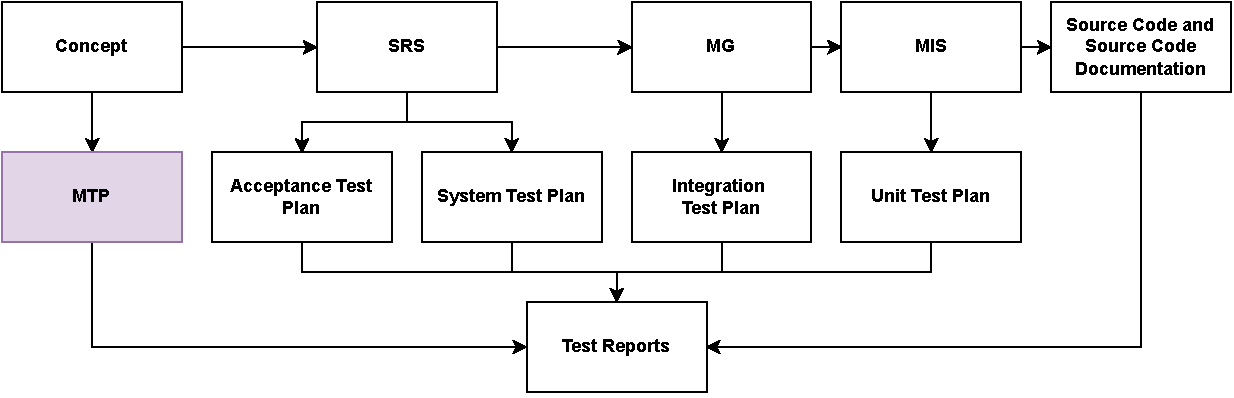
\includegraphics[width=\textwidth]{figures/mtpOrg.pdf}
    \caption{Dependencies Between \progname{}'s SDAs (MTP Highlighted)}
    \label{fig:dependencies}
\end{figure}

\begin{table}[!h]
    \renewcommand{\arraystretch}{1.2}
    \centering
    \caption{Location of V \& V Plans for \progname{}'s SDAs}
    \label{tab:verificationPlanLocation}
    \begin{tabular}{P{0.38\linewidth}P{0.5\linewidth}}
        \toprule
        \textbf{SDA} & \textbf{Location of V \& V Plan} \\

        \midrule

        \colourRow Concept Summary & -- \\

        Master Test Plan & Master Test Plan \\

        \colourRow Software Requirements Specification & Master Test Plan \\

        Module Guide & Master Test Plan \\

        \colourRow Module Interface Specification & Master Test Plan \\

        System, Integration, and Unit Test Plan & Master Test Plan \\

        \colourRow Acceptance Test Plan & Master Test Plan \\

        Source Code and Source Code Documentation& System, Integration, and
        Unit Test Plan \newline Acceptance Test Plan \\

        \bottomrule
    \end{tabular}
\end{table}
\vspace*{\fill}

\subsection{Relevant Documentation}
The Master Test Plan (MTP) refers to the following Software Development
Artifacts (SDAs):
\begin{itemize}

    \item \textbf{Title}: Concept Summary for \progname{}: A Computational
    Model of Emotion for Enhancing Non-Player Character Believability in Games
    \\
    \textbf{Location}:
    \href{https://github.com/GenevaS/EMgine/blob/main/docs/ConceptSummary/EMgine_ConceptSummary.pdf}{https://github.com/GenevaS/EMgine/blob/main/docs/ConceptSummary/\newline
     EMgine\_ConceptSummary.pdf} \\
    \textbf{Description}: Product of the concept definition process. An
    overview of \progname{} purpose, design goals, and motivation.

    \item \textbf{Title}: Software Requirements Specification for \progname{}:
    A Computational Model of Emotion for Enhancing Non-Player Character
    Believability in Games \\
    \textbf{Location}:
    \href{https://github.com/GenevaS/EMgine/blob/main/docs/SRS/EMgine_SRS.pdf}{https://github.com/GenevaS/EMgine/blob/main/docs/SRS/EMgine\_SRS.pdf}
     \\
    \textbf{Description}: Product of the requirements analysis process.
    \progname{}'s problem domain, purpose, underlying models, requirements
    (functional and nonfunctional), and likely changes.

    \item \textbf{Title}: Module Guide for \progname{}: A Computational Model
    of Emotion for Enhancing Non-Player Character Believability in Games \\
    \textbf{Location}:
    \href{https://github.com/GenevaS/EMgine/blob/main/docs/Design/MG/EMgine_MG.pdf}{https://github.com/GenevaS/EMgine/blob/main/docs/Design/MG/\newline
     EMgine\_MG.pdf} \\
    \textbf{Description}: Product of the architecture definition process. An
    overview of \progname{}'s architecture and component modules.

    \item \textbf{Title}: Module Interface Specification for \progname{}: A
    Computational Model of Emotion for Enhancing Non-Player Character
    Believability in Games \\
    \textbf{Location}: TDB \\
    \textbf{Description}: Product of the design definition process.
    Specifications of each module in \progname{} such that they are readily
    implementable.

    \item \textbf{Title}: Source Code and Documentation for \progname{}: A
    Computational Model of Emotion for Enhancing Non-Player Character
    Believability in Games \\
    \textbf{Location}: TDB \\
    \textbf{Description}: Product of the implementation process. A
    software-based realization of \progname{}'s requirements and design,
    accompanied by documentation of the resulting components and/or processes.

    \item \textbf{Title}: User Manual for \progname{}: A Computational Model
    of Emotion for Enhancing Non-Player Character Believability in Games \\
    \textbf{Location}: TDB \\
    \textbf{Description}: Product of the implementation process. A document
    written for \progname{}'s users to help them learn about and use
    \progname{}.

\end{itemize}

\noindent \progname{} has additional test plan documents as follows:
\begin{itemize}

    \item \textbf{Title}: System, Integration, and Unit Test Plan for
    \progname{}: A Computational Model of Emotion for Enhancing Non-Player
    Character Believability in Games \\
    \textbf{Location}: TDB \\
    \textbf{Description}: Test specifications to evaluate \progname{}'s models
    with respect to its design specifications (see
    Section~\ref{plan:implementation}).

    \clearpage\item \textbf{Title}: Acceptance Test Plan for \progname{}: A
    Computational Model of Emotion for Enhancing Non-Player Character
    Believability in Games \\
    \textbf{Location}: TDB \\
    \textbf{Description}: Test specifications to evaluate the ability of
    \progname{}'s models to produce expected emotions and intensities (see
    Section~\ref{plan:validate}).

\end{itemize}

\noindent This document also refers to the:
\begin{itemize}

    \item IEEE Standard for Software and System Test Documentation (IEEE
    Std 829-2008)~\citep{vvDocIEEE} to inform the creation of this document,
    the System, Integration, and Unit Test Plan, and the Acceptance Test Plan

    \item IEEE Standard for System, Software, and Hardware Verification and
    Validation (IEEE Std 1012-2016)~\citep{vvIEEE} to inform the creation of
    this document and the System, Integration, and Unit Test Plan

    \item IEEE Recommended Practice for Software Requirements Specifications
    (IEEE Std 830-1998 (R2009))~\citep{srsIEEE} to inform the evaluation of
    \progname{}'s Software Requirements Specification (SRS)

    \item ISO/IEC/IEEE International Standard - Systems and software
    engineering -- System life cycle processes (ISO/IEC/IEEE
    15288:2015(E))~\citep{slcIEEE} to inform the evaluation of \progname{}'s
    design

\end{itemize}

\subsection{Testing and Verification Tools}\label{sec:tools}
\progname{}'s development uses the C\# programming language because it is one
of the languages supported in Unity, a well-known game development
platform~\citep{unity3Dcsharp}. The supporting Integrated Development
Environment (IDE), Microsoft Visual Studio (VS), is the default script editor
in Unity. \progname{} development uses VS 2022 (Community Edition), which can
access the following tools:
\begin{itemize}

    \item \textbf{NUnit Unit Testing Framework} \\
    This supports the bulk of the automated testing approach for unit,
    integration, system, and regression testing. The IDE is configured to
    automatically run existing unit tests when it is compiling the code base.
    Unity Testing Framework uses custom integration of NUnit
    3.5~\citep{unity3Dtestingfw}.

    \item \textbf{Moq Library for .NET} \\
    This supports tests that rely on components that do not have a concrete
    implementation, such as the user-defined data types
    %(Section~\ref{sec_sysUserDataTypes}).
    It allows the definition of mocked
    interface calls within unit tests that are type-safe~\citep{moq}.

    \item \textbf{Performance Analysis} \\
    \progname{} uses the performance tools built into VS 2022, which includes
    CPU, memory, and time usage tools~\citep{vs2022perf}.

    \item \textbf{Code Style and Quality Analyzers} \\
    \progname{}'s development uses the official .NET Compiler Platform
    (Roslyn)~\citep{roslyn} and the third-party Roslynator~\citep{roslynator}
    analyzers to help adhere to good code quality and style practices. The
    Unity documentation also references Roslyn analyzers for code style and
    quality~\citep{unity3Droslyn}.

\end{itemize}